\documentclass[]{spie}  %>>> use for US letter paper
%\documentclass[a4paper]{spie}  %>>> use this instead for A4 paper
%\documentclass[nocompress]{spie}  %>>> to avoid compression of citations

\renewcommand{\baselinestretch}{1.0} % Change to 1.65 for double spacing

\usepackage{amsmath,amsfonts,amssymb}
\usepackage{graphicx}
\usepackage[colorlinks=true, allcolors=blue]{hyperref}

\title{Principal component analysis of the Chandra/ACIS gain}
\author[a]{Hans Moritz G\"unther}
\author[b]{Akos Bogdan}
\author[b]{Nick Durham }
\affil[a]{MIT Kavli Institute for Astrophysics and Space Research, Massachusetts Institute of Technology, Cambridge, MA 02139, USA}
\affil[b]{Smithsonian Astrophysical Observatory, Cambridge, MA 02139, USA}

\authorinfo{Send correspondence to H.M.G. (E-mail: hgunther@mit.edu)}


% Option to view page numbers
\pagestyle{empty} % change to \pagestyle{plain} for page numbers
\setcounter{page}{301} % Set start page numbering at e.g. 301

\begin{document}
\maketitle

\begin{abstract}
Up to 2020, the Chandra/ACIS gain has been calibrated using the External Calibration Source (ECS). The ECS consists of a radioactive material and is placed in the ACIS housing such that all chips are fully illuminated. Since the radioactive source decays over time, count rates are becoming too low. Instead, astrophysical calibration sources will be needed, which do not fill the field of view. Here, we determine the dominant spatial components through principal component analysis (PCA). We find that, given the noise levels observed today, all ACIS gain maps can be sufficiently described by just a few (often only one) spatial components. We conclude illuminating a small area is sufficient for gain calibration. We apply this to observations of the astrophysical source Cas A. The resulting calibration is found to be accurate to 0.6\% in at least 68\% of the chip area, following the same definition for the calibration accuracy that has been used since launch.
\end{abstract}

% Include a list of keywords after the abstract
\keywords{Chandra, calibration, gain, principal component analysis}

% Use cite and citenum

\section{INTRODUCTION}
\label{sec:intro}
X-ray astronomy has been revolutionized by the advent of CCD detectors. With CCDs, we can determine the energy of every single incoming photon and thus extract and X-ray spectrum at any position of the image. In this way, spectra of many point sources such as a young stellar cluster, or of different positions in the an extended source, e.g.\ a suerpnova remnant can be obtained in just a single pointing. However, CCDs do not directly output the photon energy. When an X-ray photon hits the CCD, it generates and electron cloud in the detector material. THe number of electrons in that cloud is related to the photon energy. However, electrons can be lost if either the cloud spreads over too many pixels or if they are trapped on defects, causing a chanrge-trasfer inefficiency (CTI) [REF HERE]. Even after the electrons are read out, the signal needs to be amplified and processed electronically, until a PHA (Pulse hieght amplitude) value for a specific event is recorded. This PHA value is roughly linearly realted to the photon energy, but the exact realtion needs to be calibrated empirically using a source of photons of known energy.

In for the ACIS detector [REF] on the Chandra X-ray Observatory, this calibration has long relied on the so called ``external calibration source'' (ECS). The ECS consists of a Fe-55 source and aluminum and titanium targets, thus emitting strong Al K$\alpha$, and Ti and Mn K$\alpha$ and K$\beta$ lines in addition to a number of weaker lines. The source is mounted such that it illuminates all ACIS chips uniformly while they are stowed during radiation belt passage.

In the past, the dPHA maps for each chip have been constructed by fitting a number of regions (256 regions of 32 * 128 pixels each) independently. One can see that the maps show consistent large scale structure. As the calibration source ages, fitting 256 regions independently is not be possibly any longer; instead we could try to parameterize the spatial dependence and fit just a few parameters which can be done with more noisy data.

The basic idea is to use PCA (Principal Component Analysis). Each observed dPHA image can be thought of as a vector with 256 features. PCA will find new bases vectors in 256 dimensional space choosing the bases vectors (=image components) such that most of the variability between images can be described by just a few components.

Code is available at ...

Use term GAIN somewhere

In the analysis, it will be apprarent that the chips fall into three groups, where the BI chips behave similarly, I0 and I2 do, and the remaining FI chips form the last group. Most of the plots are thus done for just one or a few chips (e.g. I0, I1, and S3).

The gain also depends strongly on temperature, but that is beyond the scope of this study, all data here is from nominal cold observations.


\section{CALIBRATION DATA}
Data from the ECS has been used since Chandra's launch to calibrate the relation between PHA and photon energy. We reduce the data follwing the same established procedures. First, data is reprocessed with the standard \texttt{acis\_process\_events} procedure to correcting for CTI, but not for the gain, since this is the quantity that we want to establish. Events are split by chip and within each ship in regions of $32*128$~pixels, which gives 256 regions per chip. For each region, a spectrum is extracted and the position of the Al, Ti, and Mn K$\alpha$ lines are fit, see Figure~\ref{fig:example} for an example.
\begin{figure} [ht]
  \begin{center}
    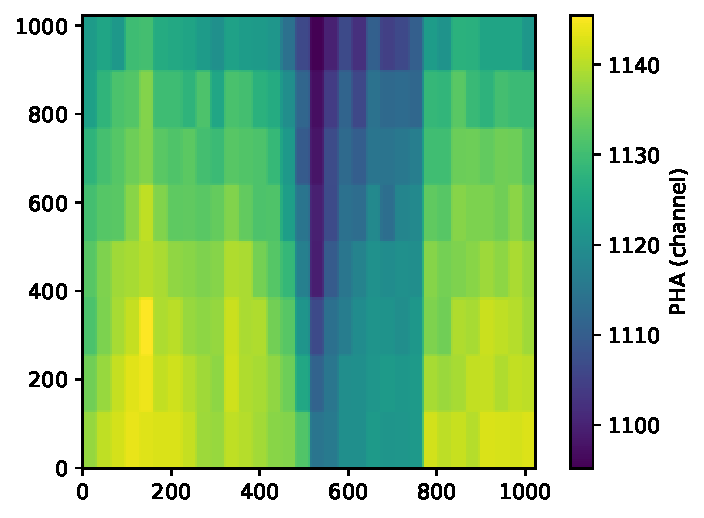
\includegraphics[height=5cm]{figures/i1e50Ti.pdf}
  \end{center}
  \caption
      {Measured PHA values on the I3 chip in the Ti line in epoch 50 \label{fig:example}. The x and y axis are given in pixels.
}
\end{figure}
In this procedure the fits for each tile on the chip are totally independent. Yet, Figure~\ref{fig:example} shows that large scale structure exists. First, we can discern the node boundaries. In node 3 (x pixel values 513-768) the PHA value if the Ti line peak is significantly lower than in the other three nodes. Furthermore, there is a clear trend with higher PHA values towards the bottom of the figure (smaller y pixel values).

Smaller regions would a allow a more fine-grained picture of the spatial dependence of the gain calibration. However, each region needs to a have a sufficient number of ECS counts to extract a spectrum and fit the position of the emission lines. If the number of counts is too low, then the fit might be unsuccessful or the statistical uncertainties of the fitted value are large. Even for the tiles chosen, this problem occurs since the count rate from the ECS declines as the Fe-55 source decays over time. Until 2015, the gain calibration was performed every three months. Since 2016, data for six month is combined to ensure a sufficient count number to sucessfully fit the line position in the spectrum. Even with this adjustment, it happens that in some regions the number of counts is too low to fit the spectrum. In these cases, we fill in the missing values from the average of the neighboring tiles. No tiles ever needed filling on the S3 chip, while 260 missing values were filled on the S0 chip.

\section{PRINCIPAL COMPONENT ANALYSIS}
Principal Component analysis (PCA) is a well known mathematical concept and a description can be found elsewhere. We are using the implementation from scikit-learn\cite{scikit-learn}. In short, we can look at the 256 regions in each image as a vector in 256-d space. PCA finds a new set of basis vectors and orders them such that the first vector in the list describes the direction with the largest variance between the input data points, the second vector the direction with the second most variance and so on. The new basis vectors always form an orthogonal basis (i.e.\ the PCA components are independent) and the process of calculating them is determinisitic. (There are alternative implementations of PCA that make use of approximations to speed up the computation, but that is not a concern for the size of this dataset.) However, the new basis may not be complete. If only 215 datapoints are put into the PCA, the new basis will only have 215 vectors and thus not span the entire 256 dimensional space. PCA can be used as a tool for dimensionality reduction and noise reduction. A simple example is a set of datapoints in 3D space that all fall onto a single plane with just some noise above and below the plane. In that case, the PCA will return two vectors that span up the plane and one that's perpendicular to it. The importance of this last component will be small. We can then decide to discard this component and only retain the remaining two, effectively forcing all points on the plane, which reduces the noise in one direction. At the end, those new noise-reduced points can be projected back into the original 3D space.

Similarly, we use PCA here to identify spatial components of the gain that vary together. For example, if the gain for the four nodes on the chip evolves with time, but in a different way, then we would get four components, one for each node. The images of those components would show the node in question and have a value of "0" for the others.

A few technicalities for the PCA that are worth writing down here: The mean of the data is subtracted before running PCA and the sign of the new bases vectors is arbitrary.

This description of a 256d vector discards the 2D structure of the image, no relation between individual components is assumed in the PCA. As we will see below, folding the 256-d vectors back into an $32 * 8$ image will result in sensible 2D images. This is a useful sanity check.

For each chip, we run one PCA on data from all epochs and all three lines (Al, Ti, Mn) that we can measure from the ECS. The PCA returns components that describe most of the observed variance. For each point in time (epoch) and line (Al, Ti, Mn), we get a set of factors. Time evolution in the gain thus is described by the time series of these coefficients.

\begin{figure} [ht]
  \begin{center}
    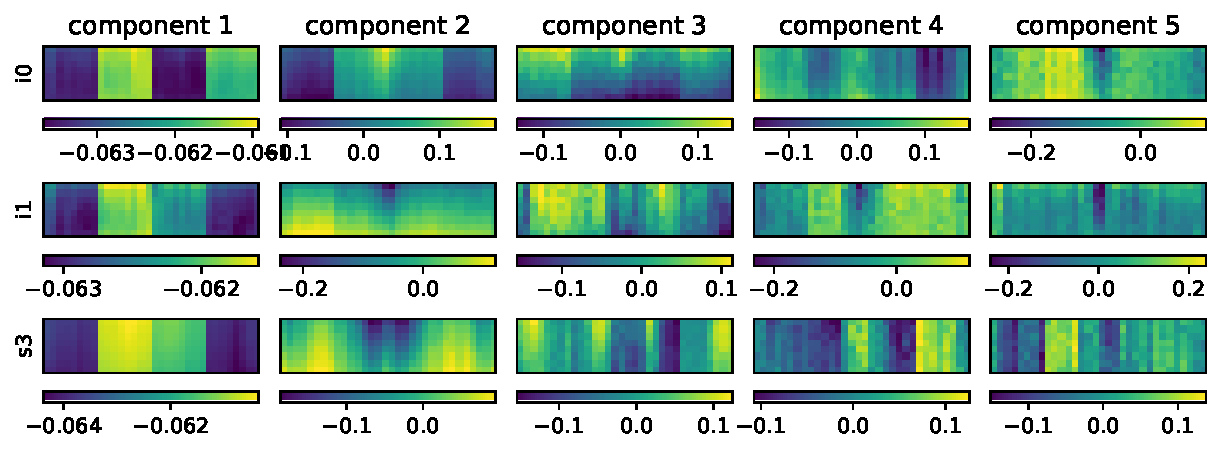
\includegraphics[height=5cm]{figures/components.pdf}
  \end{center}
  \caption
      {Most important PCA components (left to right) for different chips (rows). Some similarities are seen between chips. \label{fig:components}}
\end{figure}

The most important PCA components are shown in Figure~\ref{fig:components} for different chips. Some similarities are seen between chips. The most important component (left column) has a very small range of values, the difference between the min and max in the image of this component is only of order 0.02, while it is 0.2 to 0.5 for the other components. That means that all regions on the chip behave very similar when this component changes. We will see later that this component is essentially the linear scaling between photon energy and PHA. That proportionality differs slightly between nodes and ever more slightly within a node. The next components all have structure mostly along columns, with consistent changes from the top to the bottom of the chip
(recall that the sign is arbitrary here, since only the product of the scaling for this component $x_i$ and the 256-d vector of component values $C_i$ matter: $x_i * C_i = -x_i * -C_i$).

In most cases, spatial structure is clearly evident in these components, indication that they indeed have some physical relevance. (Remember that the PCA by itself does not know anything about the 2D structure. Each "image" is simply a 1D vector of 256 numbers.)

For comparison, Figure~\ref{fig:components_minor} shows some components of lesser importance, which look dominated by noise although some features that are spatially consistent (e.g.\ the step between the third and forth node in the top left image) are still present.

\begin{figure} [ht]
  \begin{center}
    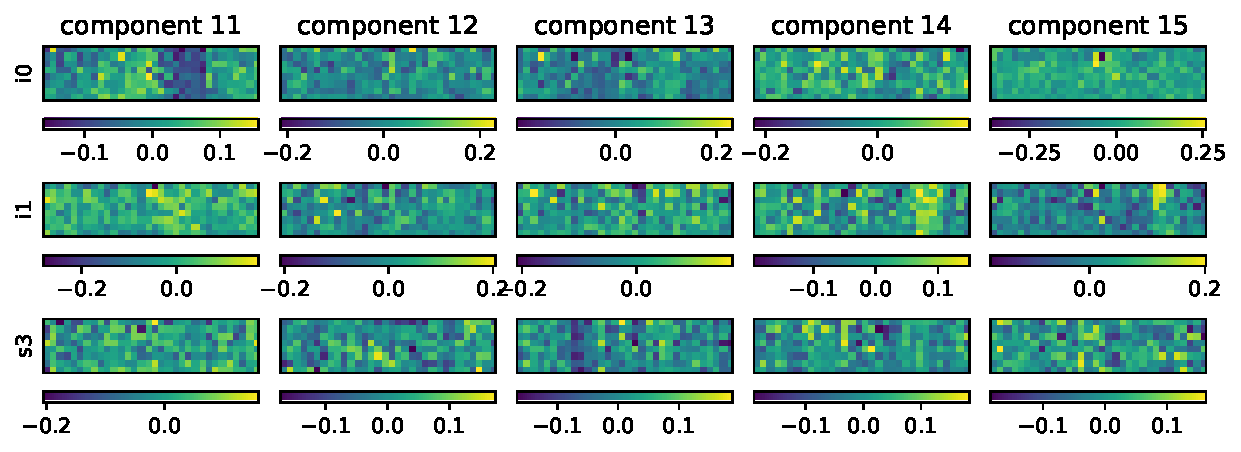
\includegraphics[height=5cm]{figures/components_minor.pdf}
  \end{center}
  \caption
      {Most important PCA components (left to right) for different chips (rows). Some similarities are seen between chips. \label{fig:components_minor}}
\end{figure}

\subsection{Explained variance and time evolution of scaling factors}
Slide Type

The PCA orders components by importance, such that the first component explained the most of the data variance. Thus, one of the first things to look at is how many components are needed to describe, e.g.\ 95\% of the observed variance. Given that the observations do contain noise, we are not looking for a perfect description of the input data by PCA components. Instead, we need to determine which components are physical and which just fit the noise.

Also, we want to look at the time dependence of the scaling factors for the most important components.


\acknowledgments
Support
for this work was provided in part through NASA grant NNX17AG43G and
Smithsonian Astrophysical Observatory (SAO) contract SV3-73016 to MIT
for support of the {\em Chandra} X-Ray Center (CXC), which is operated
by SAO for and on behalf of NASA under contract NAS8-03060.
The
analysis uses Astropy, a community-developed core Python
package for Astronomy\cite{astropy1,astropy2}, numpy\cite{numpy}, scikit-learn\cite{scikit-learn} and
IPython\cite{IPython}. Displays are done with
matplotlib\cite{matplotlib} and bokeh\cite{bokeh}.
% References
\bibliography{report} % bibliography data in report.bib
\bibliographystyle{spiebib}

\end{document}
